% File: jupiter-css-c306.tex
% CSS lattice for jupiter-sequence-diagram-c306.tex

\documentclass{standalone}

% preamble for jupiter-paper related TikZ drawing
\usepackage{tikz}
\usetikzlibrary{shapes, positioning, arrows.meta, calc, backgrounds, fit}

% default horizontal/vertical distance
\def\hdist{1.5}
\def\vdist{1.5}

\newcommand{\state}[2]{% #1: state label; #2: position
  \node (#1) [circle, inner sep = 0pt, minimum size = 10mm, text width = 10mm, align = center, draw, #2, font = \Large] {$#1$};
}

\newcommand{\transition}[4][]{% #2: start state; #3: end state; #4: transition label; #1: transition label position (optional)
  \draw[>=Stealth, ->] (#2) to node [rectangle, draw, above = 2pt, sloped, #1] {#4} (#3);
}

\tikzset{node distance = \vdist and \hdist}
\tikzset{path/.style = {draw, rounded corners, very thick, #1}}


\begin{document}
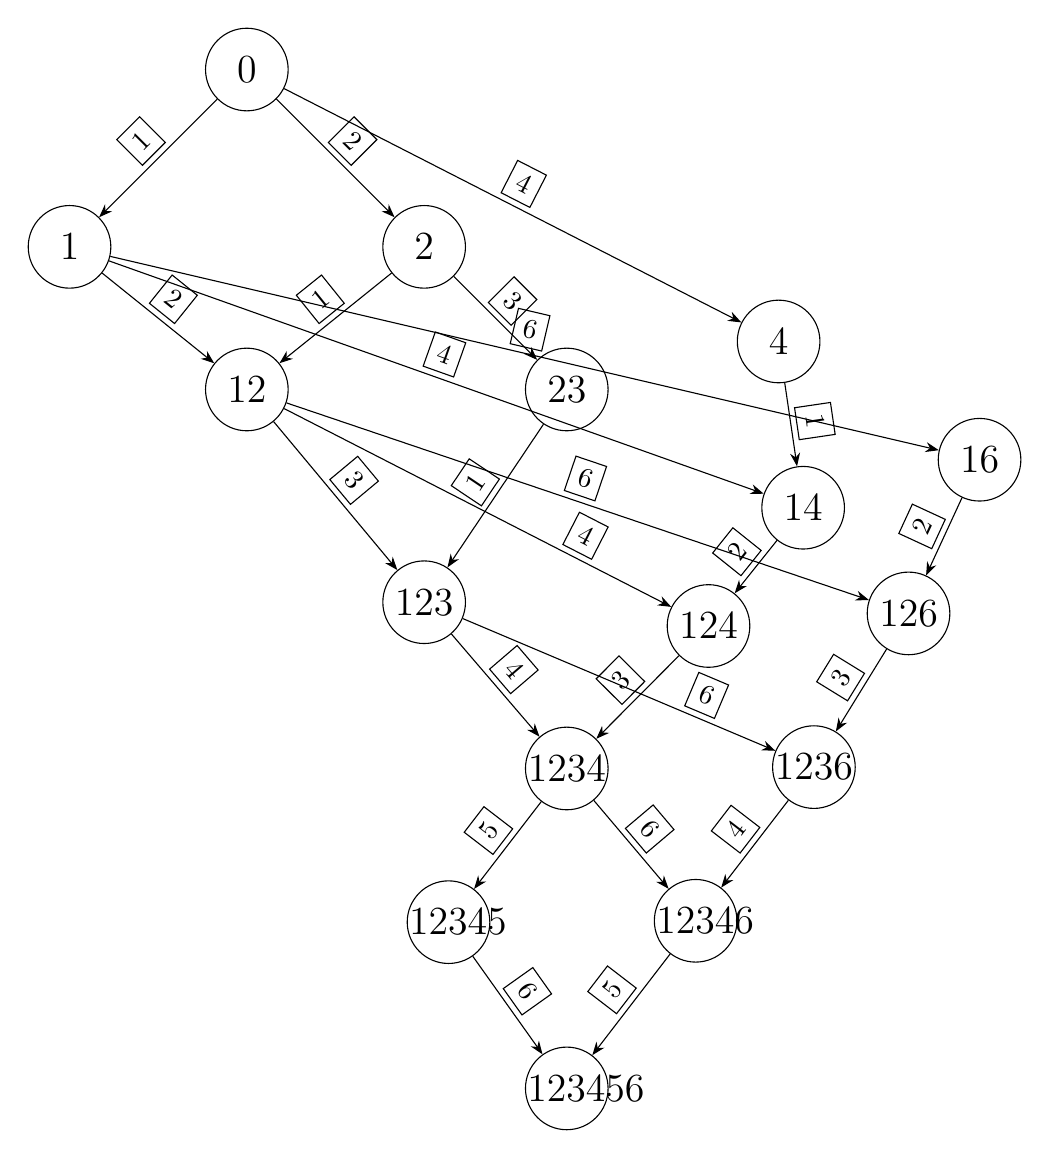
\begin{tikzpicture}
  \state{0}{}
  \state{1}{below left = of 0}
  \state{2}{below right = of 0}
  \state{12}{below = 2*\vdist of 0}
  \transition{0}{1}{1}
  \transition{0}{2}{2}
  \transition{1}{12}{2}
  \transition{2}{12}{1}

  \state{23}{right = 2*\vdist of 12}
  \state{123}{below = 2.3*\vdist of 2}
  \transition{2}{23}{3}
  \transition{12}{123}{3}
  \transition{23}{123}{1}

  \state{4}{below right = 0.3*\vdist and 2.5*\hdist of 2}
  \state{14}{below right = 0.50*\vdist and 1.5*\hdist of 23}
  \state{124}{below left = 0.50*\vdist and 0.30*\hdist of 14}
  \state{1234}{below = 2.5*\vdist of 23}
  \transition{0}{4}{4}
  \transition{1}{14}{4}
  \transition{4}{14}{1}
  \transition[near end]{12}{124}{4}
  \transition{14}{124}{2}
  \transition{123}{1234}{4}
  \transition{124}{1234}{3}

  \state{12345}{below left = 0.80*\vdist and 0.5*\hdist of 1234}
  \transition{1234}{12345}{5}

  \state{16}{below right = 0.50*\vdist and 1.2*\hdist of 4}
  \state{126}{below left = 0.80*\vdist and 0.1*\hdist of 16}
  \state{1236}{below left = 0.80*\vdist and 0.3*\hdist of 126}
  \state{12346}{below left = 0.80*\vdist and 0.5*\hdist of 1236}
  \state{123456}{below = 2.0*\vdist of 1234}

  \transition{1}{16}{6}
  \transition{12}{126}{6}
  \transition{16}{126}{2}
  \transition[near end]{123}{1236}{6}
  \transition{126}{1236}{3}
  \transition{1234}{12346}{6}
  \transition{1236}{12346}{4}
  \transition{12345}{123456}{6}
  \transition{12346}{123456}{5}
\end{tikzpicture}
\end{document}
